\documentclass[dvips,slidetop,mathserif,brown]{beamer}

\usepackage[utf8]{inputenc}
\usepackage[T1]{fontenc}
\usepackage{amsmath}
\usepackage{lmodern}
\usepackage[british]{babel}
\usepackage{graphicx}
\usepackage{url}
\usepackage{verbatim}
\usepackage[all]{xy}
\usepackage{dpf}

\usetheme{Singapore}
\usecolortheme{lily}
\setbeamertemplate{navigation symbols}{}

\definecolor{lily}{rgb}{0.7,0.2,0.2}
\definecolor{grey}{rgb}{0.9,0.9,0.9}
\definecolor{dgreen}{rgb}{0.0,0.47,0.0}
\newxyColor{dgreen}{0.0 0.47 0.0}{rgb}{}

\hypersetup{
  pdftitle={Model-driven engineering in RDF - a way to version control},
  pdfauthor={Hans Georg Schaathun and Adrian Rutle},
  pdfsubject={Presentation at NIK 2018}
}

\graphicspath{{images/}}

\begin{document}

\title{Model-driven engineering in RDF - a way to version control}% \footnote{Courtesy to Alessandro Rossini}}

\subject{Model-driven engineering in RDF - a way to version control}

\author[Adrian Rutle]{Hans Georg Schaathun\inst{1} \and \underline{Adrian Rutle}\inst{2}}

\institute[Western Norway University of Applied Sciences]{\inst{1} NTNU Norwegian University of Science and Technology, Ålesund \and
\inst{2} Western Norway University of Applied Sciences, Bergen}

\date[19 Sept 2018]{19$^{th}$ September 2018}

% \logo{\includegraphics[width=5em]{../../../common/logos/uib_logo}}

\section{Introduction}

\begin{frame}
  \titlepage
\end{frame}

% \begin{frame}{Short story of my life}
%   \begin{itemize}
%     \item \begin{tabular}{p{4.5em} l}\emph{1980} & Born in San Benedetto del Tronto, Italy\end{tabular}
%     \pause
%     \item \begin{tabular}{p{4.5em} l}\emph{1999-2003} & Bachelor in Informatics, University of L'Aquila\end{tabular}
%     \pause
%     \item \begin{tabular}{p{4.5em} l}\emph{2004-2006} & Master in Informatics, University of L'Aquila\end{tabular}
%     \item[] \begin{tabular}{p{4.5em} l} & Exchange student, University of Bergen\end{tabular}
%     \pause
%     \item \begin{tabular}{p{4.5em} l}\emph{2007} & Software engineer\end{tabular}
%     \pause
%     \item \begin{tabular}{p{4.5em} l}\emph{2008-2011} & PhD candidate, University of Bergen\end{tabular}
%   \end{itemize}
% \end{frame}

\begin{frame}{}
  \begin{center}
    \begin{Huge}
      \textbf{Software development}
    \end{Huge}
  \end{center}
\end{frame}

\begin{frame}[containsverbatim]{Assembly coding}
  \begin{tiny}
    \begin{verbatim}
init:
mov bx,offset doors
xor ax,ax
mov cl,032h

initloop:
mov [bx],ax
inc bx
inc bx
dec cl
jnz initloop

dodoor:
xor cx,cx
mov bx,offset doors-1

doorloop:
add bx,cx
add bx,cx
inc bx
mov [bx],0FFh
inc cl
cmp cl,0Ah
jnz doorloop

programend:
cli
hlt
jmp programend

doors:
    \end{verbatim}
  \end{tiny}
\end{frame}

\begin{frame}[containsverbatim]{Imperative programming}
  \begin{footnotesize}
    \begin{verbatim}
PROGRAM DOORS

  INTEGER, PARAMETER :: n = 100
  INTEGER :: i, j
  LOGICAL :: door(n) = .TRUE.

  DO i = 1, n
    DO j = i, n, i
      door(j) = .NOT. door(j)
    END DO
  END DO

  DO i = 1, n
    WRITE(*,"(A,I3,A)", ADVANCE="NO") "Door ", i, " is "
    IF (door(i)) THEN
      WRITE(*,"(A)") "closed"
    ELSE
      WRITE(*,"(A)") "open"
    END IF
  END DO

END PROGRAM DOORS
    \end{verbatim}
  \end{footnotesize}
\end{frame}

\begin{frame}[containsverbatim]{Object-oriented programming}
  \begin{footnotesize}
    \begin{verbatim}
public class HundredDoors {
    public static void main(String[] args) {
        boolean[] doors = new boolean[101];
        for (int i = 1; i <= 100; i++) {
            for (int j = 1; j <= 100; j++) {
                if(j % i == 0) doors[j] = !doors[j];
            }
        }
        for (int i = 1; i <= 100; i++) {
            System.out.printf("Door %d:
              %s%n", i, doors[i] ? "open" : "closed");
        }
    }
}
    \end{verbatim}
  \end{footnotesize}
\end{frame}

\begin{frame}{Modelling}
  \begin{center}
    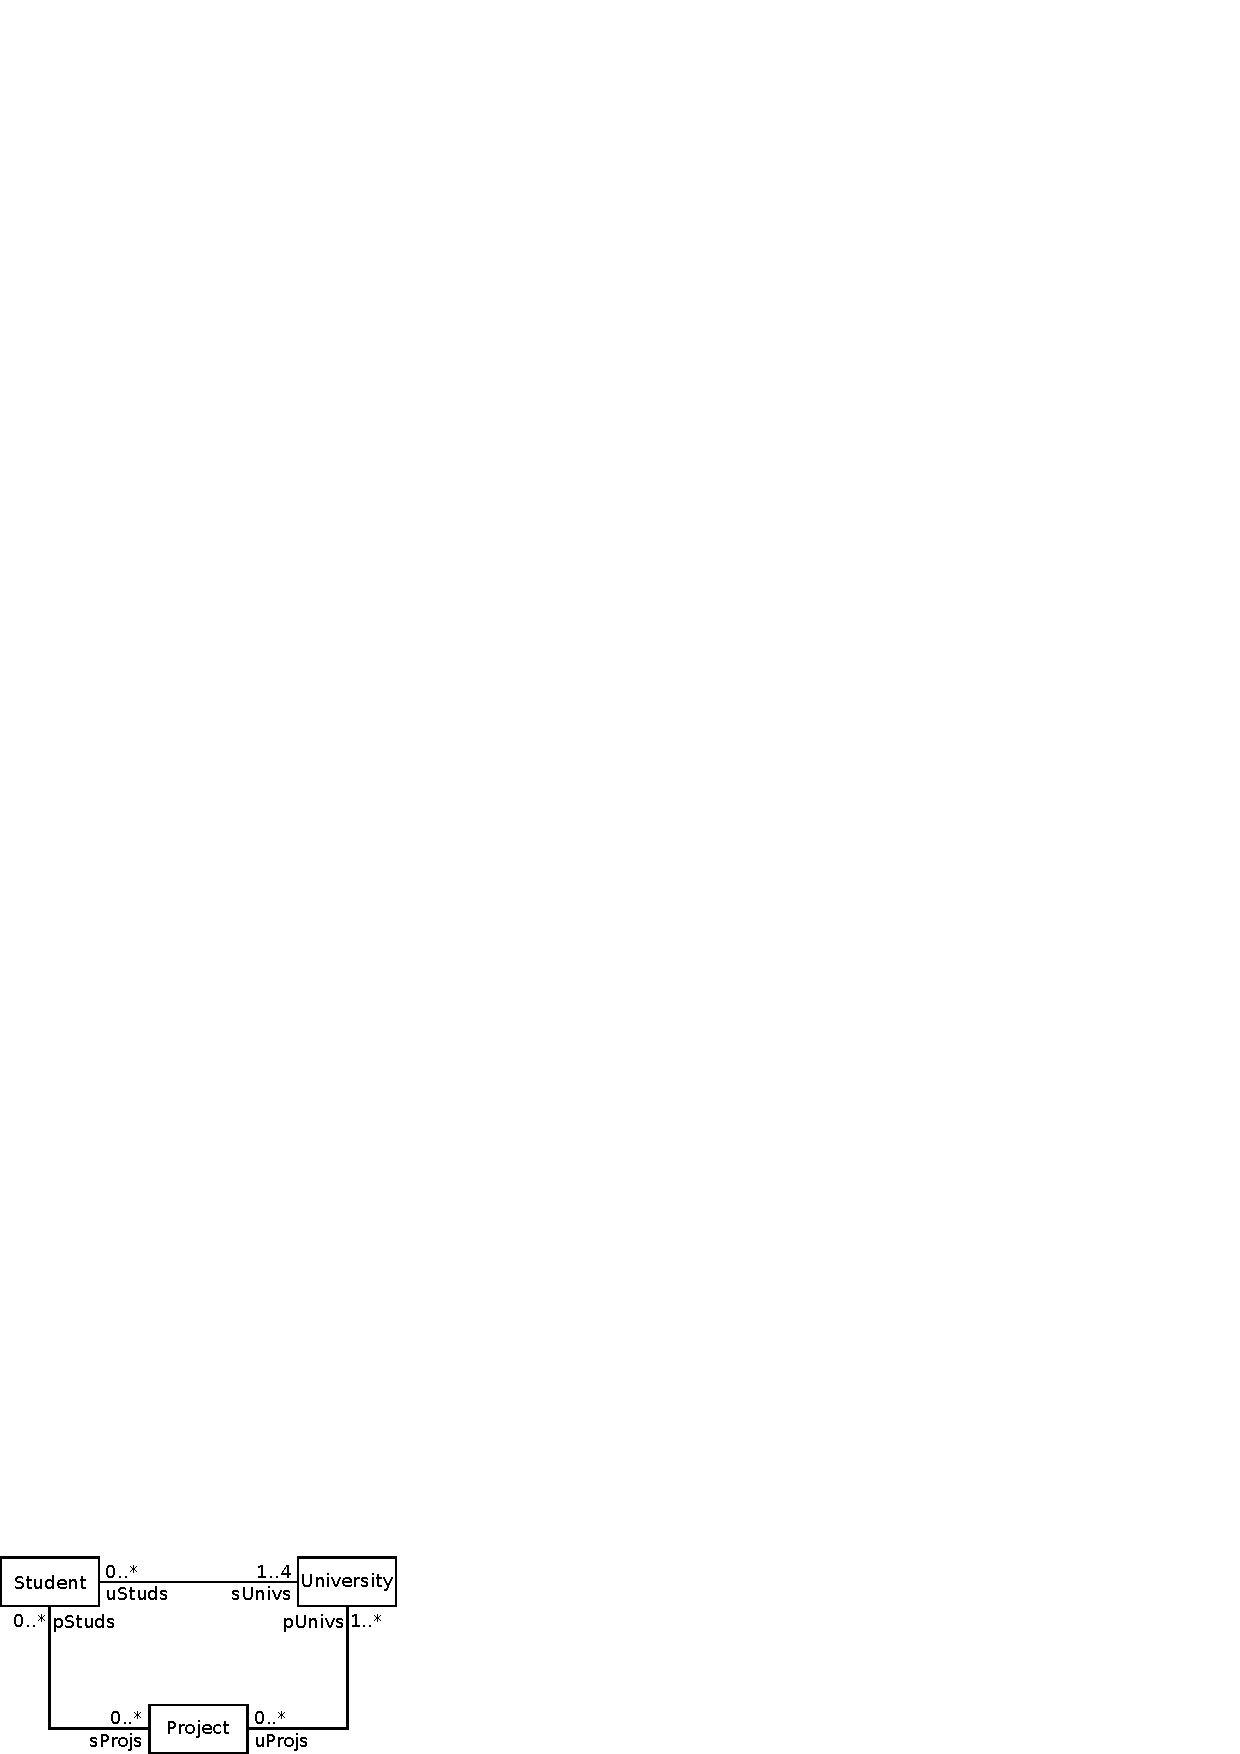
\includegraphics{ex_project_uml_class_3}
  \end{center}
\end{frame}

\begin{frame}{Model}
  ``An abstraction of a system allowing predictions or inferences to be made.''
\end{frame}

\begin{frame}{}
  \begin{center}
    \begin{Huge}
      \textbf{Software engineering}
    \end{Huge}
  \end{center}
\end{frame}

\begin{frame}{}
  \begin{columns}[T]
    \column{.5\textwidth}
    \begin{block}{Software engineering process}
      \includegraphics<1>{process_se_1}
      \includegraphics<2>{process_se_2}
      \includegraphics<3>{process_se_3}
    \end{block}
  \end{columns}
\end{frame}

\begin{frame}{}
  \begin{center}
    \begin{Huge}
      \textbf{Model-driven engineering}
    \end{Huge}
  \end{center}
\end{frame}

\begin{frame}{}
  \begin{columns}[T]
    \column{.5\textwidth}
    \begin{block}{Software engineering process}
      \includegraphics{process_se_3}
    \end{block}
    \column{.5\textwidth}
    \begin{block}{MDE process}
      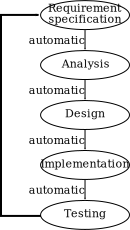
\includegraphics{process_mde}
    \end{block}
  \end{columns}
\end{frame}

\begin{frame}{MDE standards}
  \begin{itemize}
    \item Graph-based modelling languages
    \begin{itemize}
      \item Unified Modeling Language (UML)
      \item Eclipse Modeling Framework (EMF)
    \end{itemize}
    \item Text-based constraint languages
    \begin{itemize}
      \item Object Constraint Language (OCL)
    \end{itemize}
  \end{itemize}
\end{frame}

\defverbatim[colored]\oclcode{
  \begin{footnotesize}
    \begin{verbatim}
context Project
inv:
  self.pUnivs.uStuds->
    includesAll(self.pStuds)
    \end{verbatim}
  \end{footnotesize}
}

\begin{frame}[t]{Project management in UML/OCL}
  \begin{columns}[T]
    \column{0.5\textwidth}
    \begin{block}{UML class diagram}
      \includegraphics<1>[width=\textwidth]{ex_project_uml_class_0}
      \includegraphics<2-3>[width=\textwidth]{ex_project_uml_class_1}
      \includegraphics<4-5>[width=\textwidth]{ex_project_uml_class_2}
      \includegraphics<6-7>[width=\textwidth]{ex_project_uml_class_3}
      \includegraphics<8>[width=\textwidth]{ex_project_uml_class_4}
      \includegraphics<9>[width=\textwidth]{ex_project_uml_class_3}
    \end{block}
    \column{0.5\textwidth}
    \only<9>{
      \begin{block}{OCL constraint}
        \oclcode
      \end{block}
    }
  \end{columns}
  \begin{block}{Requirements}
    \only<1-2>{
      \begin{enumerate}
        \item[1] A university educates \emph{none} to \emph{many} students.
        \item[2] A student studies \emph{at least at one} and \emph{at most at four} universities.
      \end{enumerate}
    }
    \only<3-4>{
      \begin{enumerate}
        \item[3] A project involves \emph{none} to \emph{many} students.
      \end{enumerate}
    }
    \only<5-6>{
      \begin{enumerate}
        \item[4] A project must be controlled by \emph{at least one} university.
      \end{enumerate}
    }
    \only<7->{
      \begin{enumerate}
        \item[5] A student involved in a project must study at \emph{at least one} of the controlling universities.
      \end{enumerate}
    }
  \end{block}
\end{frame}

\section{Diagram Predicate Framework}

\begin{frame}{}
  \begin{center}
    \begin{Huge}
      \textbf{Diagram Predicate Framework}
    \end{Huge}
  \end{center}
\end{frame}

\begin{frame}{Diagram Predicate Framework (DPF)}
  \begin{itemize}
    \item Diagrammatic specification framework founded on category theory and graph transformation
    \begin{itemize}
      \item diagrammatic modelling
      \item metamodelling
      \item model transformation
      \item model versioning
      \item deep metamodelling
    \end{itemize}
  \end{itemize}
\end{frame}

% \begin{frame}{DPF's history}
%   \begin{itemize}
%     \item \begin{tabular}{p{4.5em} l}\emph{2003--} & Uwe Wolter and Yngve Lamo\end{tabular}
%     \item[] \begin{tabular}{p{4.5em} l} & Generalized Sketches\end{tabular}
%     \pause
%     \item \begin{tabular}{p{4.5em} l}\emph{2006-2010} & Adrian Rutle\end{tabular}
%     \item[] \begin{tabular}{p{4.5em} l} & (meta)modelling and model transformation\end{tabular}
%     \pause
%     \item \begin{tabular}{p{4.5em} l}\emph{2008-2011} & Alessandro Rossini\end{tabular}
%     \item[] \begin{tabular}{p{4.5em} l} & model versioning and deep metamodelling\end{tabular}
%     \pause
%     \item \begin{tabular}{p{4.5em} l}\emph{2010-2011} & Øyvind Bech, Dag Viggo Lokøen\end{tabular}
%     \item[] \begin{tabular}{p{4.5em} l} & tool support\end{tabular}
%     \pause
%     \item \begin{tabular}{p{4.5em} l}\emph{2010-2013} & Florian Mantz\end{tabular}
%     \item[] \begin{tabular}{p{4.5em} l} & metamodel evolution\end{tabular}
%     \pause
%     \item \begin{tabular}{p{4.5em} l}\emph{2011-2014} & Xiaoliang Wang\end{tabular}
%     \item[] \begin{tabular}{p{4.5em} l} & correctness of model transformation\end{tabular}
%   \end{itemize}
% \end{frame}

% \begin{frame}[t]{Project management in DPF}
%   \begin{block}{Specification}
%     \centering
%     \includegraphics<1>[scale=0.8]{ex_project_spec_0}
%     \includegraphics<2-3>[scale=0.8]{ex_project_spec_1}
%     \includegraphics<4-5>[scale=0.8]{ex_project_spec_2}
%     \includegraphics<6-7>[scale=0.8]{ex_project_spec_3}
%     \includegraphics<8>[scale=0.8]{ex_project_spec_4}
%   \end{block}
%   \begin{block}{Requirements}
%     \only<1-2>{
%       \begin{enumerate}
%         \item[1] A university educates \emph{none} to \emph{many} students.
%         \item[2] A student studies \emph{at least at one} and \emph{at most at four} universities.
%       \end{enumerate}
%     }
%     \only<3-4>{
%       \begin{enumerate}
%         \item[3] A project involves \emph{none} to \emph{many} students.
%       \end{enumerate}
%     }
%     \only<5-6>{
%       \begin{enumerate}
%         \item[4] A project must be controlled by \emph{at least one} university.
%       \end{enumerate}
%     }
%     \only<7->{
%       \begin{enumerate}
%         \item[5] A student involved in a project must study at \emph{at least one} of the controlling universities.
%       \end{enumerate}
%     }
%   \end{block}
% \end{frame}

\begin{frame}[t]{Project management in DPF}
  \only<2->{
    \begin{block}{Specification}
      \centering
      \includegraphics[scale=0.8]{ex_project_spec_4}
    \end{block}
  }
  \only<3>{
    \begin{block}{Requirements}
      \begin{enumerate}
        \item[5] A student involved in a project must study at \emph{at least one} of the controlling universities.
      \end{enumerate}
    \end{block}
  }
\end{frame}

\begin{frame}[t]{}
  \begin{columns}[T]
    \column{0.5\textwidth}
    \begin{block}{Specification $\spec{S} = \specf{S}{\Sigma}$}
      \centering
      \includegraphics<1->[width=\textwidth]{ex_project_spec}
    \end{block}
    \only<4>{
      \begin{block}{Atomic constraints $\aconsts{S}\!\!:\!\sig{\Sigma}$}
        \centering
        \resizebox{\textwidth}{!}{
          \begin{tabular}{|l|c|c|}
            \hline
              \boldmath $(\pi, \delta)$ & \boldmath$\arity{\Sigma}(\pi)$ & \boldmath $\delta(\arity{\Sigma}(\pi))$ \\
            \hline
              (\mult{1}{4}, $\delta_1$) &
              $\xymatrix{1 \ar[r]^-{a} & 2}$ &
              $\xymatrix{\textspecscript{Student} \ar[rr]^-{\textspecscript{sUnivs}} & & \textspecscript{University}}$ \\
            \hline
              (\textpred{[inverse]}, $\delta_2$) &
              $\xymatrix{1 \ar@/^1em/[r]^-{a} & 2 \ar@/^1em/[l]^-{b}}$ &
              $\xymatrix{\textspecscript{Student} \ar@/^1em/[rr]^-{\textspecscript{sUnivs}} & & \textspecscript{University} \ar@/^1em/[ll]^-{\textspecscript{uStuds}}}$ \\
            \hline
              (\textpred{[surjective]}, $\delta_3$) &
              $\xymatrix{1 \ar[r]^-{a} & 2}$ &
              $\xymatrix{\textspecscript{University} \ar[rr]^-{\textspecscript{uStuds}} & & \textspecscript{Student}}$ \\
            \hline
              (\textpred{[composition]}, $\delta_4$) &
              $\xymatrix{1 \ar[r]^-{a} \ar[dr]_-{c} & 2 \ar[d]^-{b} \\ & 3}$ &
              $\xymatrix{\textspecscript{Project} \ar[rr]^-{\textspecscript{pUnivs}} \ar[drr]_-{\textspecscript{pStuds'}} & & \textspecscript{University} \ar[d]^-{\textspecscript{uStuds}} \\ & & \textspecscript{Student}}$ \\
            \hline
              (\textpred{[image-inclusion]}, $\delta_5$) &
              $\xymatrix{1 \ar@/^1em/[r]^-{a} \ar@/_1em/[r]_-{b} & 2}$ &
              $\xymatrix{\textspecscript{Project} \ar@/^1em/[rr]^-{\textspecscript{pStuds}} \ar@/_1em/[rr]_-{\textspecscript{pStuds'}} & & \textspecscript{Student}}$ \\
            \hline
          \end{tabular}
        }
      \end{block}
    }
    \column{0.5\textwidth}
    \only<2->{
      \begin{block}{Graph $\ugraph{S}$}
        \centering
        \includegraphics<2->[width=\textwidth]{ex_project_graph}
      \end{block}
    }
    \only<3->{
      \begin{block}{Signature $\sig{\Sigma} = \sigf{\Sigma}$}
        \centering
        \resizebox{\textwidth}{!}{
          \begin{tabular}{|p{7em}|c|c|p{12em}|}
            \hline
              \boldmath $\pi \in \preds{\Sigma}$ & \boldmath $\arity{\Sigma}(\pi)$ & \textbf{Proposed vis.} & \textbf{Semantic interpretation} \\
            \hline
              $\mult{m}{n}$ &
              $\xymatrix{1 \ar[r]^-{a} & 2}$ &
              $\xymatrix{\framebox[1.5em][c]{\textspecscript{X}} \ar[r]^-{\textspecscript{f}}_-{\textspecscript{[m..n]}} & \framebox[1.5em][c]{\textspecscript{Y}}}$ &
              $\forall x \in X: m \leq |f(x)| \leq n$, with $0 \leq m \leq n$ and $n \geq 1$ \\
            \hline
              \textpred{[injective]} &
              $\xymatrix{1 \ar[r]^-{a} & 2}$ &
              $\xymatrix{\framebox[1.5em][c]{\textspecscript{X}} \ar[r]^-{\textspecscript{f}}_-{\textspecscript{[inj]}} & \framebox[1.5em][c]{\textspecscript{Y}}}$ &
              $\forall x,x' \in X:$ $f(x) = f(x')$ implies $x = x'$ \\
            \hline
              \textpred{[surjective]} &
              $\xymatrix{1 \ar[r]^-{a} & 2}$ &
              $\xymatrix{\framebox[1.5em][c]{\textspecscript{X}} \ar[r]^-{\textspecscript{f}}_-{\textspecscript{[surj]}} & \framebox[1.5em][c]{\textspecscript{Y}}}$ &
              $\forall y \in Y$ $\exists x \in X: y \in f(x)$ \\
            \hline
              \textpred{[inverse]} &
              $\xymatrix{1 \ar@/^1em/[r]^-{a} & 2 \ar@/^1em/[l]^-{b}} $ &
              $\xymatrix{\framebox[1.5em][c]{\textspecscript{X}} \ar@/^1em/[r]^-{\textspecscript{f}}="f" & \framebox[1.5em][c]{\textspecscript{Y}} \ar@/^1em/[l]^-{\textspecscript{g}}="g" \ar@/^/@{-}"f";"g"_-{\textspecscript{[inv]}}}$ &
              $\forall x \in X$ , $\forall y \in Y: y \in f(x)$ if and only if $x \in g(y)$ \\
            \hline
              \textpred{[irreflexive]} &
              $\xymatrix{1 \ar@(r,u)_-(0.4){a}}$ &
              $\xymatrix{\framebox[1.5em]{\textspecscript{X}} \ar@(r,u)_-(0.4){\textspecscript{f}}_-(0.9){\textspecscript{[irr]}}}$ &
              $\forall x \in X:$ $x \notin f(x)$ \\
            \hline
              \textpred{[composition]} &
              $\xymatrix{1 \ar[r]^-{a} \ar[dr]_-{c} & 2 \ar[d]^-{b} \\ & 3}$ &
              $\xymatrix{\framebox[1.5em][c]{\textspecscript{X}} \ar[r]^-{\textspecscript{f}} ="w" \ar[dr]_-(0.4){\textspecscript{h}}_-(0.6){\textspecscript{[comp]}} & \framebox[1.5em][c]{\textspecscript{Y}} \ar[d]^-{\textspecscript{g}} \\ & \framebox[1.5em][c]{\textspecscript{Z}}}$ &
              $\forall x \in X: h(x) = \bigcup \{g(y) \mid y \in f(x)\}$ \\
            \hline
              \textpred{[image\-inclusion]} &
              $\xymatrix{1 \ar@/^1em/[r]^-{a} \ar@/_1em/[r]_-{b} & 2}$ &
              $\xymatrix{\framebox[1.5em][c]{\textspecscript{X}} \ar@/^1em/[r]^-{\textspecscript{f}} ="f" \ar@/_1em/[r]_-{\textspecscript{g}} ="g" \ar@/^/@{->} "f";"g"_-{\textspecscript{[}\sqsubseteq\textspecscript{]}} & \framebox[1.5em][c]{\textspecscript{Y}}}$ &
              $\forall x \in X: \, f(x) \subseteq g(x)$ \\
            \hline
          \end{tabular}
        }
      \end{block}
    }
  \end{columns}
\end{frame}

\begin{frame}{Project management instance}
  \begin{center}
    \includegraphics[scale=0.8]{ex_project_spec_inst}
  \end{center}
\end{frame}

\section{Model versioning}

\begin{frame}{}
  \begin{center}
    \begin{Huge}
      \textbf{Model versioning}
    \end{Huge}
  \end{center}
\end{frame}

% \begin{frame}{Pessimistic versioning}
%   \begin{itemize}
%     \item Shared artefacts for all developers
%     \begin{itemize}
%       \item \emph{lock-modify-unlock}
%     \end{itemize}
%     \item Separate modifications (One at a time)
%   \end{itemize}
% \end{frame}

\begin{frame}{Optimistic versioning}
  \begin{itemize}
    \item Local copy of artefacts for each developer
    \begin{itemize}
      \item centralised (\emph{copy-modify-merge})
      \item distributed
    \end{itemize}
    \item Simultaneous modifications
  \end{itemize}
\end{frame}

\begin{frame}{Centralised optimistic versioning}
  \begin{columns}[T]
    \column{.33\textwidth}
    \begin{block}{Repository}
      \includegraphics<1-4>[width=\textwidth]{ex_project_vc_standard_spec_v1}
      \includegraphics<5-9>[width=\textwidth]{ex_project_vc_standard_spec_v2}
      \includegraphics<10-12>[width=\textwidth]{ex_project_vc_standard_spec_v3}
    \end{block}
    \column{.33\textwidth}
    \begin{block}{Alice's copy}
      \includegraphics<2>[width=\textwidth]{ex_project_vc_standard_spec_v1}
      \includegraphics<3-7>[width=\textwidth]{ex_project_vc_standard_spec_v2}
      \includegraphics<8-10>[width=\textwidth]{ex_project_vc_standard_spec_a2}
      \includegraphics<11>[width=\textwidth]{ex_project_vc_standard_spec_md_1}
      \includegraphics<12>[width=\textwidth]{ex_project_vc_standard_spec_md_2}
    \end{block}
    \column{.33\textwidth}
    \begin{block}{Bob's copy}
      \includegraphics<6>[width=\textwidth]{ex_project_vc_standard_spec_v2}
      \includegraphics<7-12>[width=\textwidth]{ex_project_vc_standard_spec_v3}
    \end{block}
  \end{columns}
  \begin{block}{Timeline}
    \includegraphics<1>[scale=0.8]{ex_project_vc_timeline_1}
    \includegraphics<2>[scale=0.8]{ex_project_vc_timeline_2}
    \includegraphics<3>[scale=0.8]{ex_project_vc_timeline_3}
    \includegraphics<4>[scale=0.8]{ex_project_vc_timeline_4}
    \includegraphics<5>[scale=0.8]{ex_project_vc_timeline_5}
    \includegraphics<6>[scale=0.8]{ex_project_vc_timeline_6}
    \includegraphics<7>[scale=0.8]{ex_project_vc_timeline_7}
    \includegraphics<8>[scale=0.8]{ex_project_vc_timeline_8}
    \includegraphics<9>[scale=0.8]{ex_project_vc_timeline_9}
    \includegraphics<10>[scale=0.8]{ex_project_vc_timeline_10}
    \includegraphics<11>[scale=0.8]{ex_project_vc_timeline_11}
    \includegraphics<12>[scale=0.8]{ex_project_vc_timeline_12}
  \end{block}
\end{frame}

\begin{frame}{Challenges}
  \begin{itemize}
    \item Mainstream versioning systems, e.g. Subversion
    \begin{itemize}
      \item target text-based artefacts
    \end{itemize}
    \pause
    \item Prototype model versioning systems, e.g. AMOR
    \begin{itemize}
      \item lack of formal underpinning
    \end{itemize}
    \pause
    \item State-of-the-art of research
    \begin{itemize}
      \item lack of handling of constraints
    \end{itemize}
  \end{itemize}
\end{frame}

\begin{frame}{Model versioning in DPF}
  \begin{itemize}
    \item Complete work cycle
    \item Calculation and representation of differences
    \item Synchronisation
    \begin{itemize}
      \item conflict detection
      \item conflict resolution
      \item normalisation
    \end{itemize}
    \item Constraint-awareness
  \end{itemize}
  \begin{itemize}
      \item \underline{Sound formal foundation}
      \item \underline{Lacks implementation!}
      \item \centering Serialise to and rely on Resource Definition Format (RDF)
  \end{itemize}
\end{frame}


\section{Implementation in RDF}

\begin{frame}{}
  \begin{center}
    \begin{Huge}
      \textbf{Implementation in RDF}
    \end{Huge}
  \end{center}
\end{frame}

\begin{frame}[t]{DPF as RDF by example}
  \only<1->{
      \centering
      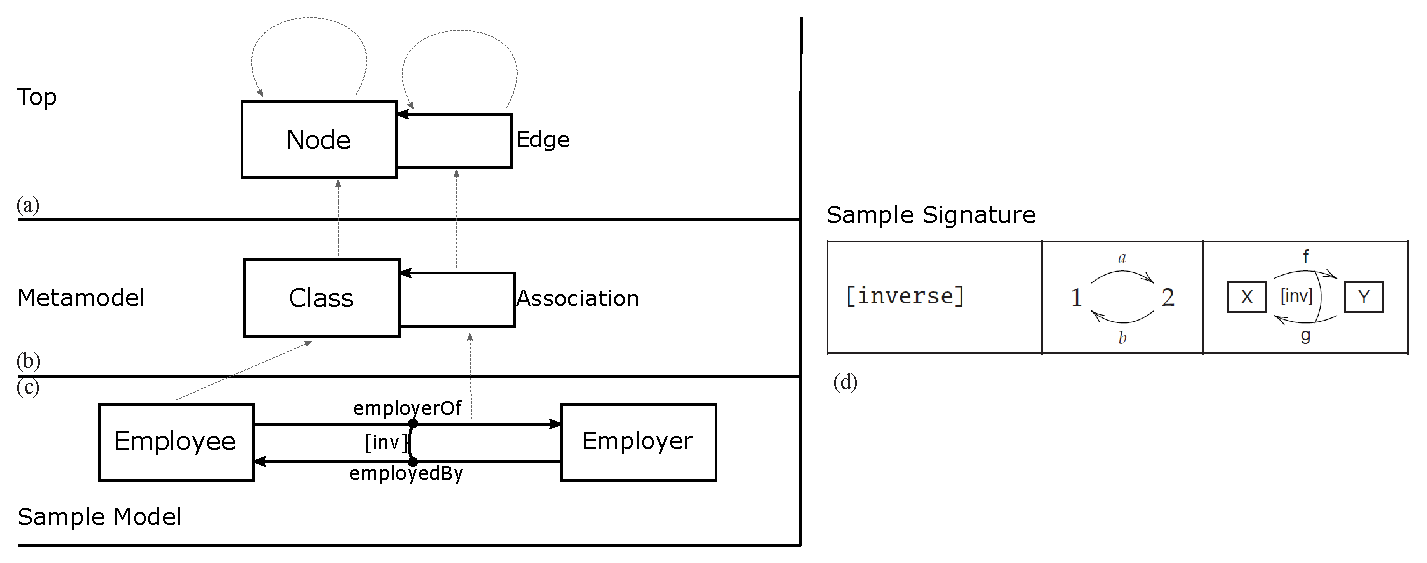
\includegraphics[scale=0.4]{ex_projects_hierarchy_new}
  }
  \only<2>{
      \centering
      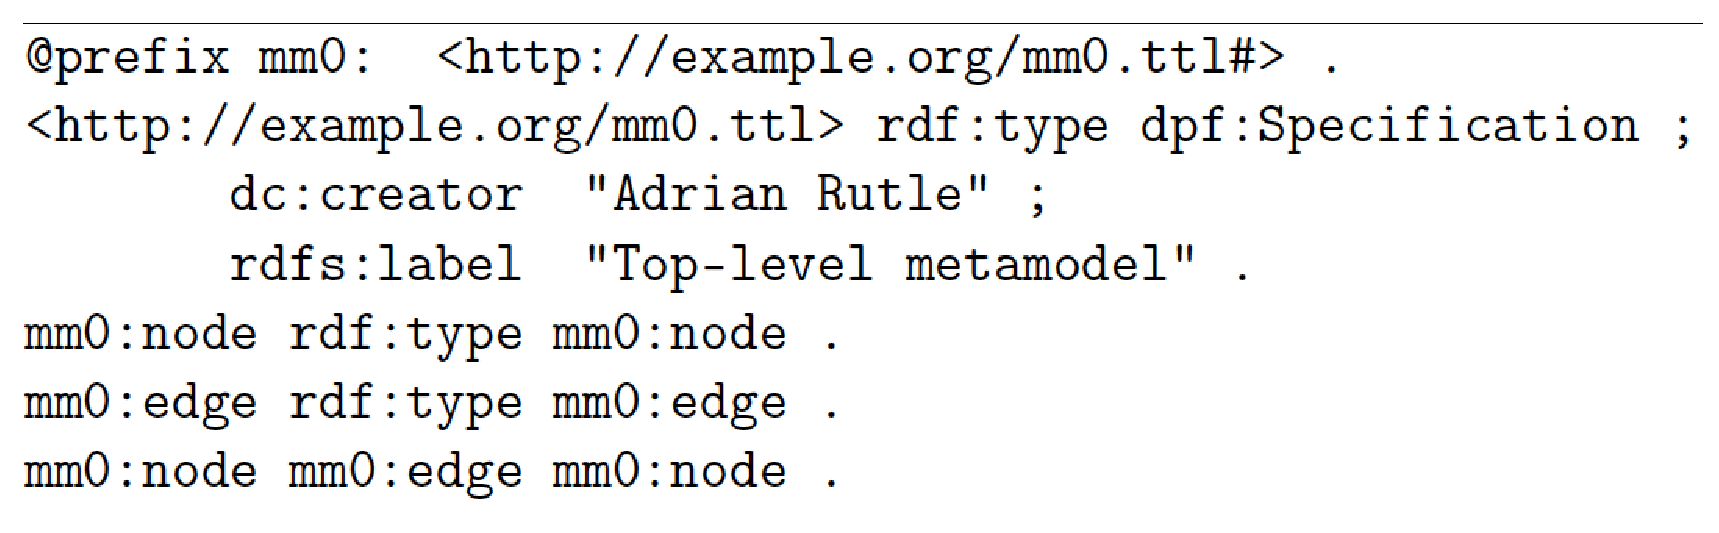
\includegraphics[scale=0.35]{top}
  }
  \only<3>{
      \centering
      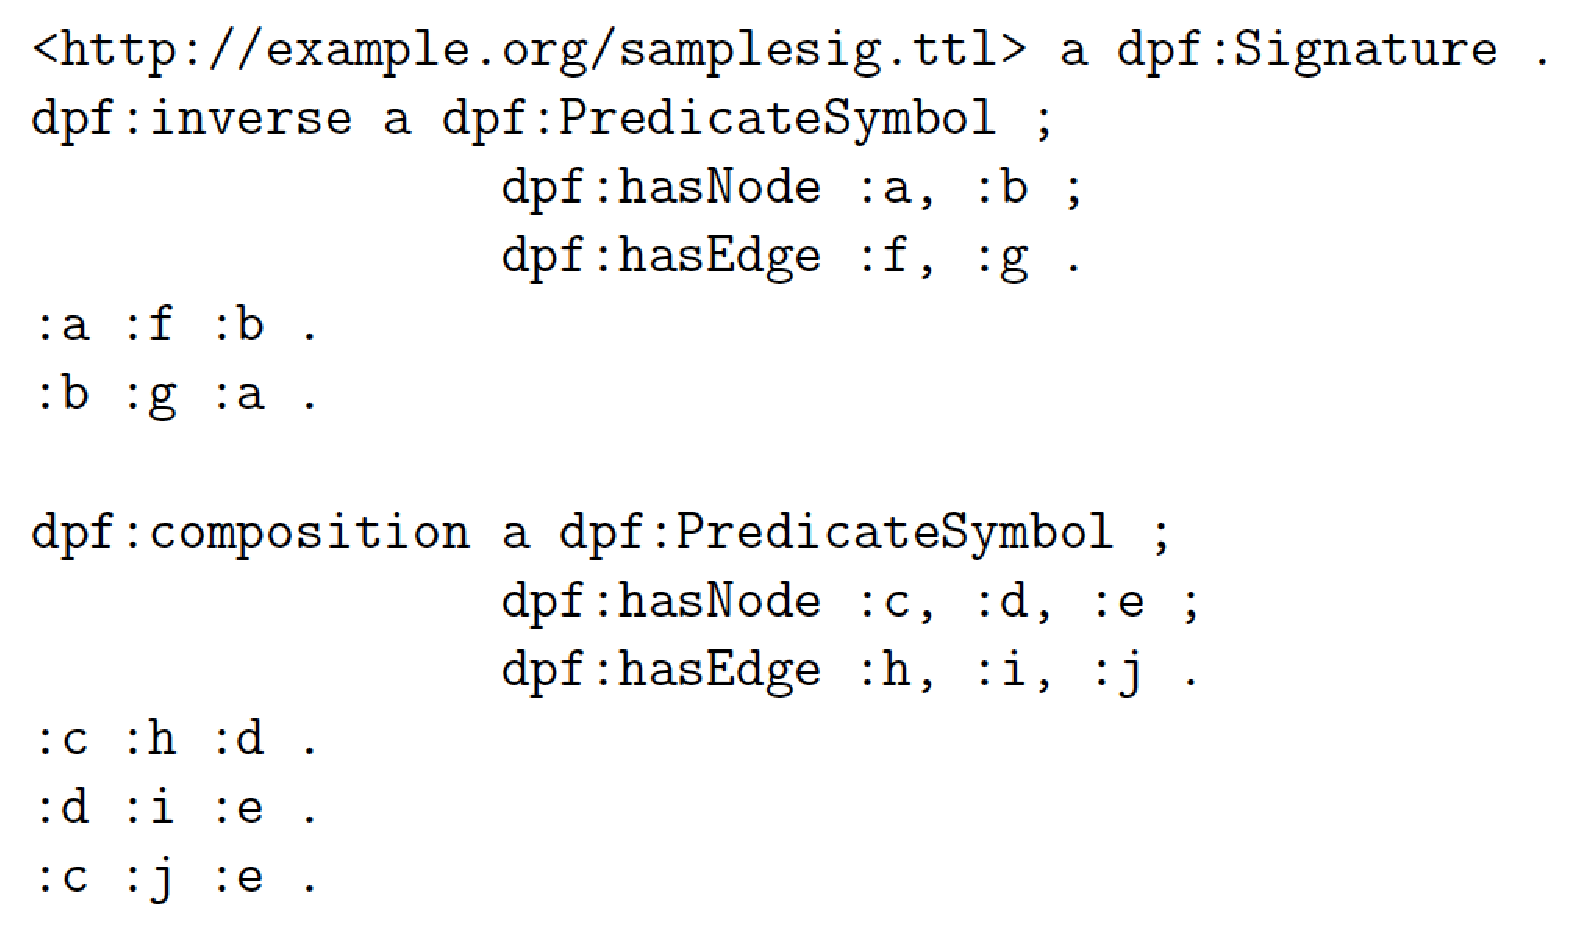
\includegraphics[scale=0.35]{sig}
  }
  \only<4>{
      \centering
      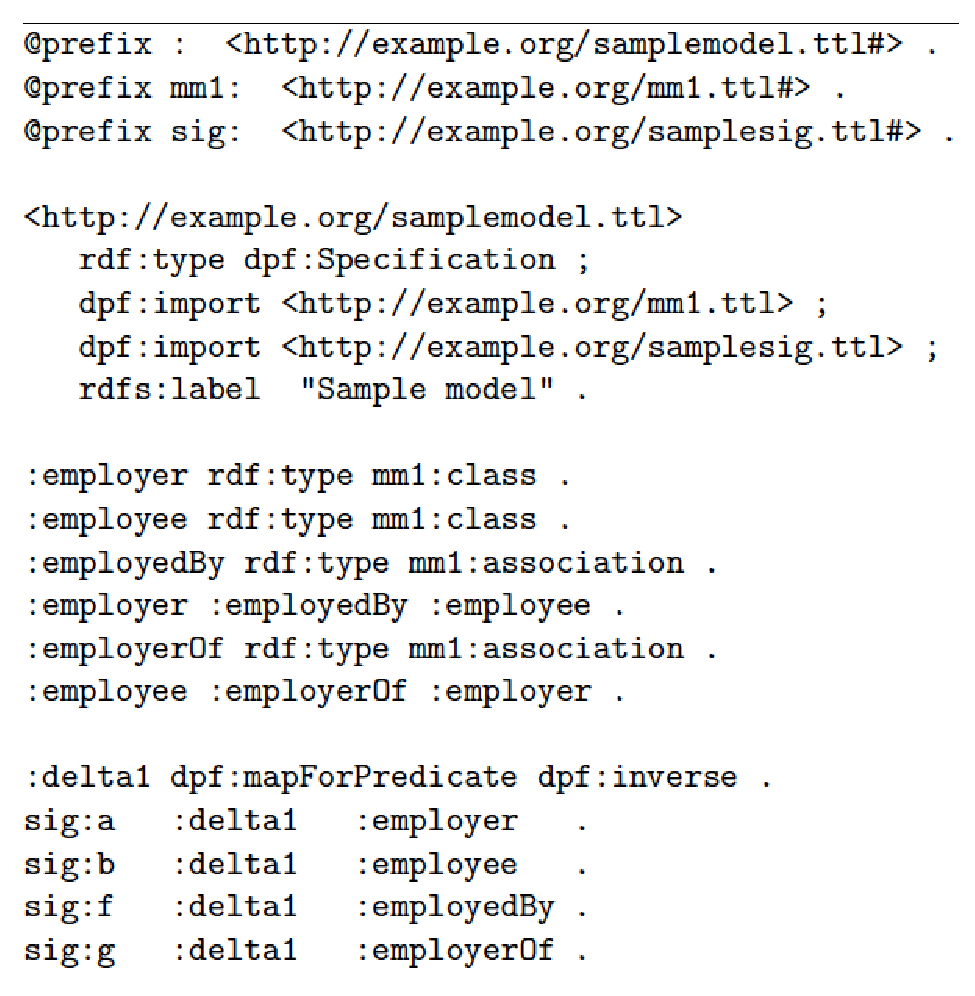
\includegraphics[scale=0.4]{inst}
  }
\end{frame}


\begin{frame}{RDF serialization}
	\begin{block}{}
		An RDF document is a set of triples
		$(s,p,o)\in(U\cup B)\times U\times(U\cup B\cup D)$, where
		$U$ is a set of URIs (universally unique identifiers),
		$B$ is a set of blind nodes (which can be viewed as local identifiers),
		and $D$ is a set of literals.
	\end{block}
	\begin{itemize}
		\item The same element may be both a vertex and an edge label
		\item The set of literals $D$, can only appear
		as a destination node of an arrow
		\item The set of vertices $V$ is not explicitly defined
		\item A vertex can only exist if it is connected to some arrow
	\end{itemize}
\end{frame}

\begin{frame}{Patch representation in RDF}
\begin{block}{}
	\begin{center}
		$\xymatrix{
			& V_0 \ar@{->}[dr]^-{(V_1\backslash V_0,V_0\backslash V_1)}   \\
			& & V_1 
		}$
	\end{center}
\end{block}
\begin{itemize}
	\item $V_0, V_1$: sets of triples
	\item $(V_1\backslash V_0,V_0\backslash V_1)$: patch representation
	\begin{itemize}
		\item $V_1\backslash V_0$: the triples to be added
		\item $V_0\backslash V_1$: the set of triples to be removed
	\end{itemize}
\end{itemize}
\end{frame}

\begin{frame}{Patch for three-way merging}
\begin{block}{}
	  \begin{center}
		$\xymatrix{
			& V_0 \ar@{->}[dr]^-{P_b}  
				\ar[dl]_-{P_a} \\
			V_a \ar[dr]^-{P_c} & & V_b \ar@{->}[dl]^-{} \\
			& V_c
		}$
	\end{center}
\end{block}
\begin{itemize}
	\item $P_a=(V_a\backslash V,V\backslash V_a)$ 
	\item $P_b=(V_b\backslash V,V\backslash V_b)$
	\item $P_c=( (V_a\backslash V)\cup(V_b\backslash V),
	(V\backslash V_a)\cup(V\backslash V_b))$: the merged patch
	\item $V_c$ is obtained by applying the patch $P_c$ to $V$.
\end{itemize}
\end{frame}


%%%%%%%%%%%%%%%%%%%%%%%%%%%%%%%% BACKUPS %%%%%%%%%%%%
\begin{comment}
\begin{frame}{}
  \begin{center}
    \begin{Huge}
      \textbf{Calculation and representation of differences}
    \end{Huge}
  \end{center}
\end{frame}

\begin{frame}{Identification of commonalities}
  \begin{center}
    $\xymatrix{
      & \spec{C} \ar@{^{(}->}[dr]^-{inc_{\spec{T}}} \ar[dl]_-{inj_{\spec{S}}} \\
      \spec{S} & & \spec{T}
    }$
  \end{center}
\end{frame}

\begin{frame}{Identification of commonalities}
  \begin{center}
    \includegraphics[scale=0.4]{ex_project_vc_standard_common}
  \end{center}
\end{frame}

\begin{frame}{Calculation of differences}
  \begin{center}
    $\xymatrix{
      & \spec{C} \ar@{^{(}->}[dr]^-{inc_{\spec{T}}} \ar@{}[dd]|-{P.O.} \ar[dl]_-{inj_{\spec{S}}} \\
      \spec{S} \ar[dr]_-{inj_{\spec{D}}} & & \spec{T} \ar@{^{(}->}[dl]^-{inc_{\spec{D}}} \\
      & \spec{D}
    }$
  \end{center}
\end{frame}

\begin{frame}{Calculation of differences}
  \begin{center}
    \includegraphics[scale=0.4]{ex_project_vc_standard_diff}
  \end{center}
\end{frame}

\begin{frame}{Representation of differences}
  \begin{center}
    \scalebox{0.8}{
      \begin{tabular}{|l|c|c|}
        \hline
          \boldmath $\theta \in \tags{G}$ & \boldmath $\arity{\Delta}(\theta)$ & \textbf{Proposed visual.} \\
        %nodes
        \hline
          $\textpred{<add>}^{N}$ &
          $1$ &
          $\textcolor{dgreen}{\framebox[1.5em][c]{\textspecscript{X}}}$ \\
        \hline
          $\textpred{<delete>}^{N}$ &
          $1$ &
          $\textcolor{red}{\framebox[1.5em][c]{\textspecscript{X}}}$ \\
        \hline
          $\rename{\textspecscript{X}}{\textspecscript{Y}}^{N}$ &
          $1$ &
          $\framebox[1.5em][c]{\textspecscript{Y}}\textspecscript{<R:X} \mapsto \textspecscript{Y>}$ \\
        \hline
          $\textpred{<conflict>}^{N}$ &
          $1$ &
          $\xymatrix{ \framebox[1.5em][c]{\textspecscript{X}} \save []*[F.]\frm{} \restore}$ \\
        \hline
        %arrows
        \hline
          $\textpred{<add>}^{A}$ &
          $\xymatrix{1 \ar[r]^-{a} & 2}$ &
          $\xymatrix{\framebox[1.5em][c]{\textspecscript{X}} \ar@*{[dgreen]}[r]^-{\textcolor{dgreen}{\textspecscript{f}}} & \framebox[1.5em][c]{\textspecscript{Y}}}$ \\
        \hline
          $\textpred{<delete>}^{A}$ &
          $\xymatrix{1 \ar[r]^-{a} & 2}$ &
          $\xymatrix{\framebox[1.5em][c]{\textspecscript{X}} \ar@*{[red]}[r]^-{\textcolor{red}{\textspecscript{f}}} & \framebox[1.5em][c]{\textspecscript{Y}}}$ \\
        \hline
          $\rename{\textspecscript{f}}{\textspecscript{g}}^{A}$ &
          $\xymatrix{1 \ar[r]^-{a} & 2}$ &
          $\xymatrix{\framebox[1.5em][c]{\textspecscript{X}} \ar[r]^-{\textspecscript{g}}_-{\textspecscript{<R:f} \mapsto \textspecscript{g>}} & \framebox[1.5em][c]{\textspecscript{Y}}}$ \\
        \hline
          $\textpred{<conflict>}^{A}$ &
          $\xymatrix{1 \ar[r]^-{a} & 2}$ &
          $\xymatrix{\framebox[1.5em][c]{\textspecscript{X}} \ar[r]^-{\textspecscript{f}} & \framebox[1.5em][c]{\textspecscript{Y}} \save [l].[]*[F.]\frm{} \restore}$ \\
        \hline
      \end{tabular}
    }
  \end{center}
\end{frame}

\begin{frame}{}
  \begin{center}
    \begin{Huge}
      \textbf{Synchronisation}
    \end{Huge}
  \end{center}
\end{frame}

\begin{frame}{Local modifications}
  \begin{center}
    \includegraphics<1>{po_ud_d_md_1}
    \includegraphics<2>{po_ud_d_md_2}
%     \includegraphics<3>[scale=0.4]{ex_project_vc_standard_spec_a2_v2_uc2}
  \end{center}
\end{frame}

\begin{frame}{Local and remote modifications}
  \begin{center}
    \includegraphics<1>{po_ud_d_md_2}
    \includegraphics<2>{po_ud_d_md_3}
  \end{center}
\end{frame}

\begin{frame}{Construct the common of commons}
  \begin{center}
    $\xymatrix{
      & & \spec{C}[B,H] \ar[dl]_-{inj_{B,i}} \ar@{^{(}->}[dr]^-{inc_{i,H}} \ar@{}[dd]|-{P.B.} \ar@/_4em/[ddll]_-{f} \ar@/^4em/@{^{(}->}[ddrr]^-{g} \\
      & \spec{C}[B,i] \ar[dl]_-{inj_B} \ar@{^{(}->}[dr]^-{inc_i} & & \spec{C}[i,H] \ar[dl]_-{inj_{i}} \ar@{^{(}->}[dr]^-{inc_{H}} \\
      \spec{V}[B] & & \spec{V}[i] & & \spec{V}[H]
    }$
  \end{center}
\end{frame}

\begin{frame}{Construct the common of commons}
  \begin{center}
    \includegraphics[width=\textwidth]{ex_project_vc_standard_common_commons}
  \end{center}
\end{frame}

\begin{frame}{Construct the difference specifications}
  \begin{center}
    \includegraphics<1>{po_ud_d_md_3}
    \includegraphics<2>{po_ud_d_md_4}
    \includegraphics<3>{po_ud_d_md_5}
  \end{center}
\end{frame}

\begin{frame}{Construct the difference specifications}
  \begin{center}
    \includegraphics[scale=0.4]{ex_project_vc_standard_ud_d}
  \end{center}
\end{frame}

\begin{frame}{Construct the merge of differences}
  \begin{center}
    \includegraphics<1>{po_ud_d_md_5}
    \includegraphics<2>{po_ud_d_md_6}
    \includegraphics<3>{po_ud_d_md_7}
  \end{center}
\end{frame}

\begin{frame}{Construct the merge of differences}
  \begin{center}
    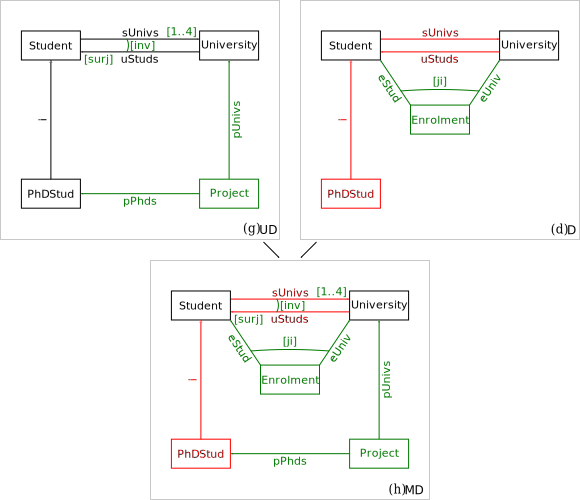
\includegraphics[scale=0.35]{ex_project_vc_standard_md}
  \end{center}
\end{frame}

\begin{frame}{Detect conflicts}
  \begin{center}
    $\xymatrix{
      \spec{{MD}} \ar@{.>}[rrr]^-{\txt{conflict detection}} & & & \spec{{MD''}}
    }$
  \end{center}
\end{frame}

\begin{frame}{Standard conflict detection rules}
  \begin{center}
    \scalebox{0.8}{
      \begin{tabular}{|c|c|c|c|}
        \hline
          Rule &
          \boldmath $\spec{L} = \spec{K}$ &
          \boldmath $\spec{R}$ \\
        %rename + delete
        \hline
          $a$ &
          $\textcolor{red}{\framebox[1.5em][c]{\textspecscript{X}}}_{\textspecscript{<R:X} \mapsto \textspecscript{Y>}}$ &
          $\xymatrix{\textcolor{red}{\framebox[1.5em][c]{\textspecscript{X}}}_{\textspecscript{<R:X} \mapsto \textspecscript{Y>}} \save [].[]*[F.]\frm{} \restore}$ \\
        \hline
          $b$ &
          $\xymatrix{\framebox[1.5em][c]{\textspecscript{X}} \ar@*{[red]}[rr]^-{\textspecscript{\textcolor{red}{f}}}_-{\textspecscript{<R:f} \mapsto \textspecscript{g>}} & & \framebox[1.5em][c]{\textspecscript{Y}}}$ &
          $\xymatrix{\framebox[1.5em][c]{\textspecscript{X}} \ar@*{[red]}[rr]^-{\textspecscript{\textcolor{red}{f}}}_-{\textspecscript{<R:f} \mapsto \textspecscript{g>}} & & \framebox[1.5em][c]{\textspecscript{Y}} \save [ll].[]*[F.]\frm{} \restore }$ \\
        %rename + rename
        \hline
          $c$ &
          $\framebox[1.5em][c]{\textspecscript{X}}^{\textspecscript{<R:X} \mapsto \textspecscript{Y>}}_{\textspecscript{<R:X} \mapsto \textspecscript{Z>}}$ &
          $\xymatrix{\framebox[1.5em][c]{\textspecscript{X}}^{\textspecscript{<R:X} \mapsto \textspecscript{Y>}}_{\textspecscript{<R:X} \mapsto \textspecscript{Z>}} \save [].[]*[F.]\frm{} \restore}$ \\
        \hline
          $d$ &
          $\xymatrix{\framebox[1.5em][c]{\textspecscript{X}} \ar[rr]^-{\textspecscript{f}}_-{\textspecscript{<R:f} \mapsto \textspecscript{g><R:f} \mapsto \textspecscript{h>}} & & \framebox[1.5em][c]{\textspecscript{Y}}}$ &
          $\xymatrix{\framebox[1.5em][c]{\textspecscript{X}} \ar[rr]^-{\textspecscript{f}}_-{\textspecscript{<R:f} \mapsto \textspecscript{g><R:f} \mapsto \textspecscript{h>}} & & \framebox[1.5em][c]{\textspecscript{Y}} \save [ll].[]*[F.]\frm{} \restore}$ \\
        %add arrow + delete node
        \hline
          $e$ &
          $\xymatrix{\textcolor{red}{\framebox[1.5em][c]{\textspecscript{X}}} \ar@*{[dgreen]}[rr]^-{\textspecscript{\textcolor{dgreen}{f}}} & & \framebox[1.5em][c]{\textspecscript{Y}}}$ &
          $\xymatrix{\textcolor{red}{\framebox[1.5em][c]{\textspecscript{X}}} \ar@*{[dgreen]}[rr]^-{\textspecscript{\textcolor{dgreen}{f}}} & & \framebox[1.5em][c]{\textspecscript{Y}} \save [ll].[]*[F.]\frm{} \restore}$ \\
        \hline
          $f$ &
          $\xymatrix{\textcolor{red}{\framebox[1.5em][c]{\textspecscript{X}}} & & \ar@*{[dgreen]}[ll]_-{\textspecscript{\textcolor{dgreen}{f}}} \framebox[1.5em][c]{\textspecscript{Y}}}$ &
          $\xymatrix{\textcolor{red}{\framebox[1.5em][c]{\textspecscript{X}}} & & \ar@*{[dgreen]}[ll]_-{\textspecscript{\textcolor{dgreen}{f}}} \framebox[1.5em][c]{\textspecscript{Y}} \save [ll].[]*[F.]\frm{} \restore}$ \\
        \hline
      \end{tabular}
    }
  \end{center}
\end{frame}

\begin{frame}{Standard conflict detection}
  \begin{center}
    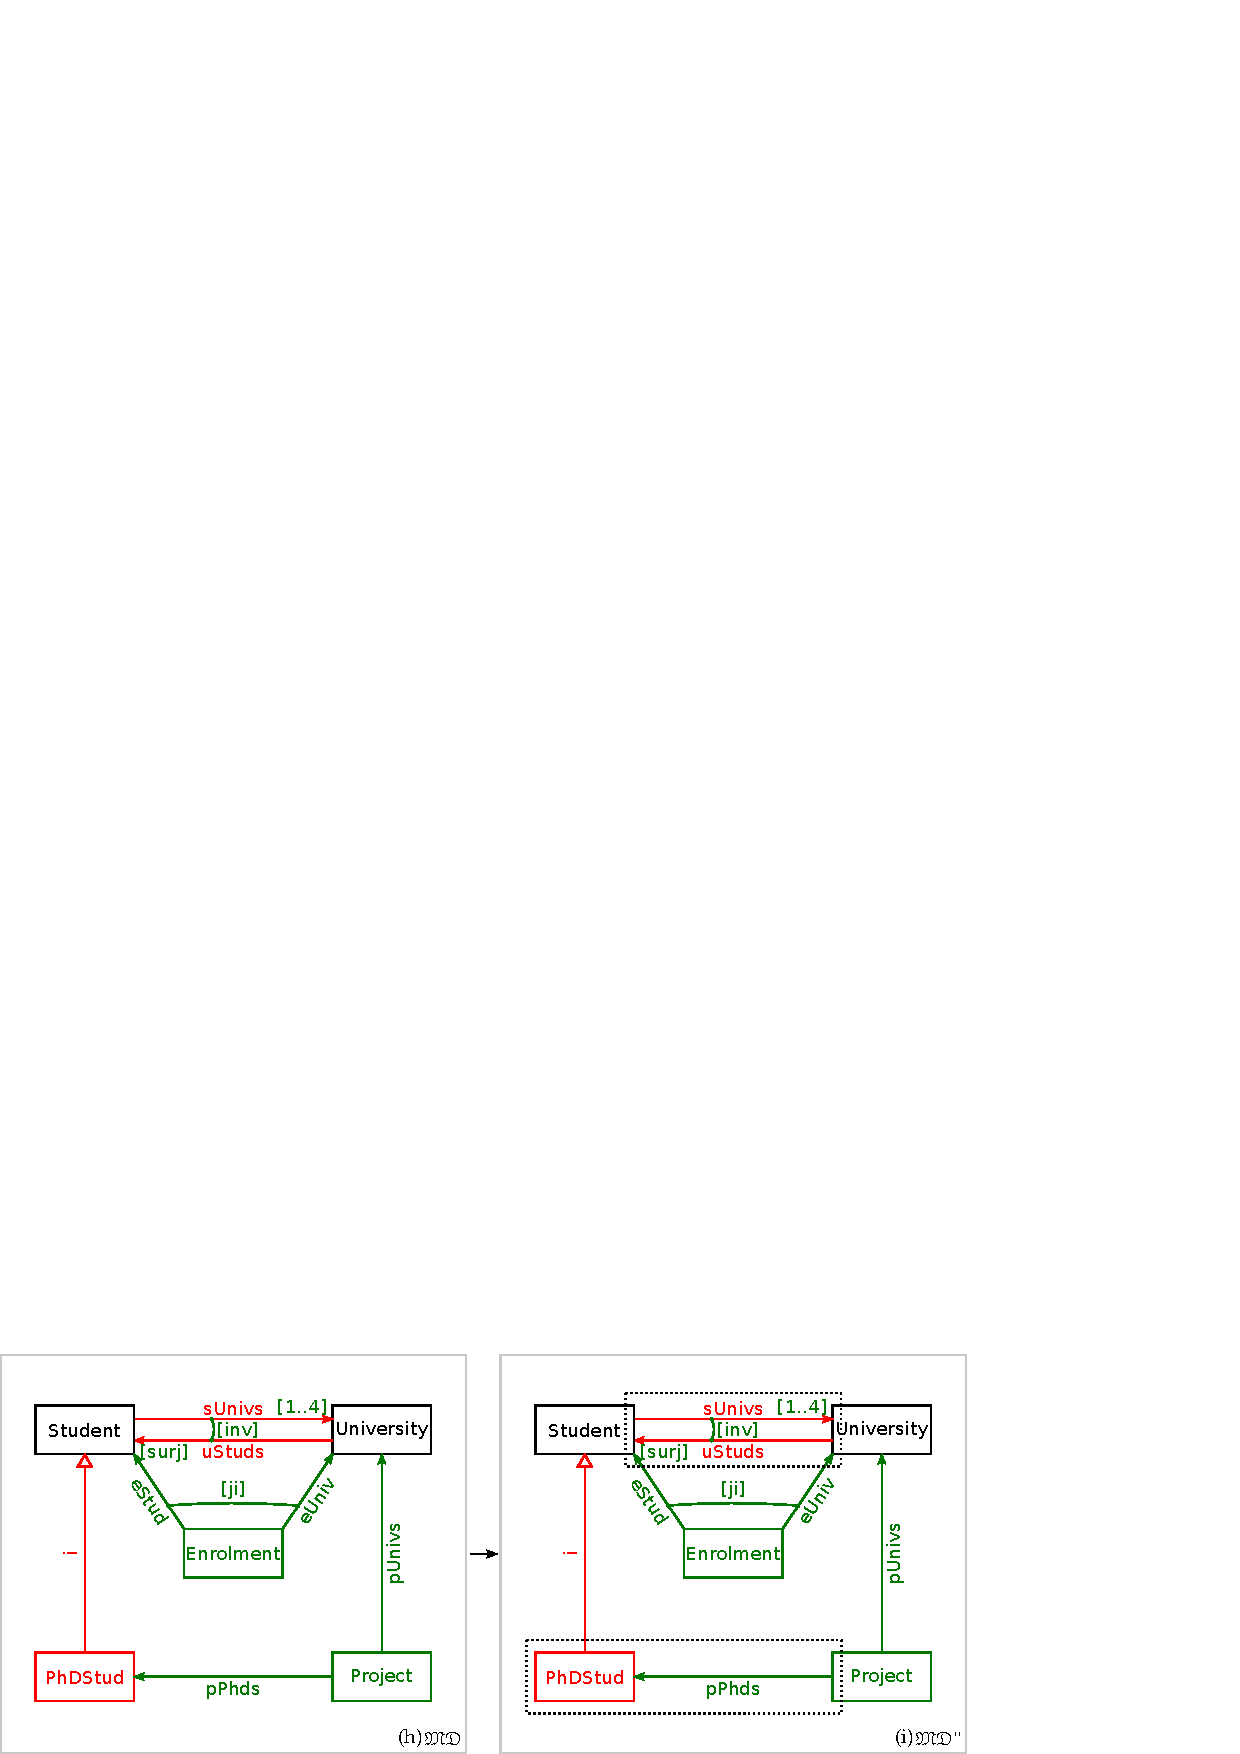
\includegraphics[width=\textwidth]{ex_project_vc_standard_md_md2}
  \end{center}
\end{frame}

\begin{frame}{Standard conflict detection}
  \begin{center}
    \includegraphics[width=\textwidth]{ex_project_vc_standard_extraction}
  \end{center}
\end{frame}

\begin{frame}{Merge of differences: Alternative scenario}
  \begin{center}
    \includegraphics[scale=0.5]{ex_project_vc_custom_md}
  \end{center}
\end{frame}

\begin{frame}{Custom conflict detection rules}
  \begin{center}
    \scalebox{0.8}{
      \begin{tabular}{|c|c|c|c|}
        \hline
          Rule &
          \boldmath $\spec{L} = \spec{K}$ &
          \boldmath $\spec{R}$ \\
        %add mult + add mult
        \hline
          $l$ &
          $\xymatrix{\framebox[1.5em][c]{\textspecscript{X}} \ar[rrr]_-{\textspecscript{f}}^-(0.3){\textspecscript{\txt<1.5em>{\textcolor{dgreen}{[$m_1$..$n_1$]}}}}^-(0.7){\textspecscript{\txt<1.5em>{\textcolor{dgreen}{[$m_2$..$n_2$]}}}} & & & \framebox[1.5em][c]{\textspecscript{Y}}}$ &
          $\xymatrix{\framebox[1.5em][c]{\textspecscript{X}} \ar[rrr]_-{\textspecscript{f}}^-(0.3){\textspecscript{\txt<1.5em>{\textcolor{dgreen}{[$m_1$..$n_1$]}}}}^-(0.7){\textspecscript{\txt<1.5em>{\textcolor{dgreen}{[$m_2$..$n_2$]}}}} & & & \framebox[1.5em][c]{\textspecscript{Y}} \save [lll].[]*[F.]\frm{} \restore}$ \\
        \hline
      \end{tabular}
    }
  \end{center}
\end{frame}

\begin{frame}{Custom conflict detection}
  \begin{center}
    \includegraphics[scale=0.5]{ex_project_vc_custom_md_md2}
  \end{center}
\end{frame}

\begin{frame}{Resolve conflicts}
  \begin{center}
    $\xymatrix{
      \spec{{MD''}} \ar@{.>}[rrr]^-{\txt{conflict resolution}} & & & \spec{{MD'''}}
    }$
  \end{center}
\end{frame}

\begin{frame}{Custom conflict resolution patterns}
  \begin{center}
    \scalebox{0.8}{
      \begin{tabular}{|c|c|c|c|}
        \hline
          Rule &
          \boldmath $\spec{L}$ &
          \boldmath $\spec{K}$ &
          \boldmath $\spec{R}$ \\
        %add mult + add mult
        \hline
          $b_L$ &
          $\xymatrix{\framebox[1.5em][c]{\textspecscript{X}} \ar[rrr]_-{\textspecscript{f}}^-(0.3){\textspecscript{\txt<1.5em>{\textcolor{dgreen}{[$m_1$..$n_1$]}}}}^-(0.7){\textspecscript{\txt<1.5em>{\textcolor{dgreen}{[$m_2$..$n_2$]}}}} & & & \framebox[1.5em][c]{\textspecscript{Y}} \save [lll].[]*[F.]\frm{} \restore}$ &
          $\xymatrix{\framebox[1.5em][c]{\textspecscript{X}} \ar[r]^-{\textspecscript{f}} & \framebox[1.5em][c]{\textspecscript{Y}}}$ &
          $\xymatrix{\framebox[1.5em][c]{\textspecscript{X}} \ar[rrr]_-{\textspecscript{f}}^-(0){\textspecscript{\txt<1.5em>{\textcolor{dgreen}{[$min(m_1,m_2)$..$max(n_1,n_2)$]}}}} & & & \framebox[1.5em][c]{\textspecscript{Y}}}$ \\
        \hline
          $b_C$ &
          $\xymatrix{\framebox[1.5em][c]{\textspecscript{X}} \ar[rrr]_-{\textspecscript{f}}^-(0.3){\textspecscript{\txt<1.5em>{\textcolor{dgreen}{[$m_1$..$n_1$]}}}}^-(0.7){\textspecscript{\txt<1.5em>{\textcolor{dgreen}{[$m_2$..$n_2$]}}}} & & & \framebox[1.5em][c]{\textspecscript{Y}} \save [lll].[]*[F.]\frm{} \restore}$ &
          $\xymatrix{\framebox[1.5em][c]{\textspecscript{X}} \ar[r]^-{\textspecscript{f}} & \framebox[1.5em][c]{\textspecscript{Y}}}$ &
          $\xymatrix{\framebox[1.5em][c]{\textspecscript{X}} \ar[rrr]_-{\textspecscript{f}}^-(0){\textspecscript{\txt<1.5em>{\textcolor{dgreen}{[$max(m_1,m_2)$..$min(n_1,n_2)$]}}}} & & & \framebox[1.5em][c]{\textspecscript{Y}}}$ \\
        \hline
      \end{tabular}
    }
  \end{center}
\end{frame}

\begin{frame}{Custom conflict resolution}
  \begin{center}
    \includegraphics[scale=0.5]{ex_project_vc_custom_md2_md3}
  \end{center}
\end{frame}

\begin{frame}{Merge of differences: Yet another alternative scenario}
  \begin{center}
    \includegraphics[scale=0.5]{ex_project_vc_custom_normalisation_md}
  \end{center}
\end{frame}

\begin{frame}{Custom conflict detection and resolution}
  \begin{center}
    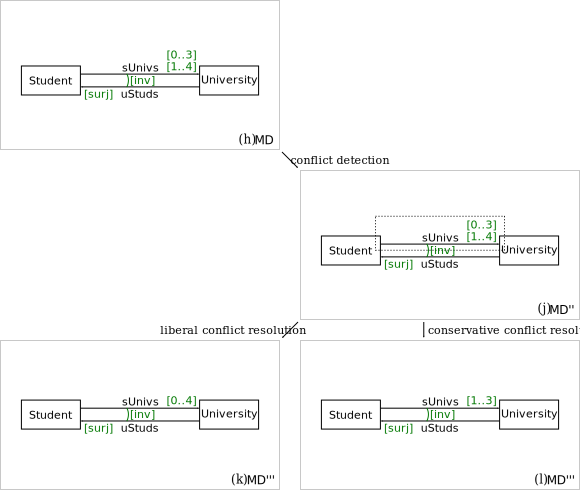
\includegraphics[scale=0.5]{ex_project_vc_custom_normalisation_md_md2_md3_1}
  \end{center}
\end{frame}

\begin{frame}{Normalise a specification}
  \begin{center}
    $\xymatrix{
      \spec{{MD}} \ar@{.>}[rr]^-{\txt{normalisation}} & & \spec{{MD'}}
    }$
  \end{center}
\end{frame}

\begin{frame}{Specification entailment}
  \begin{center}
    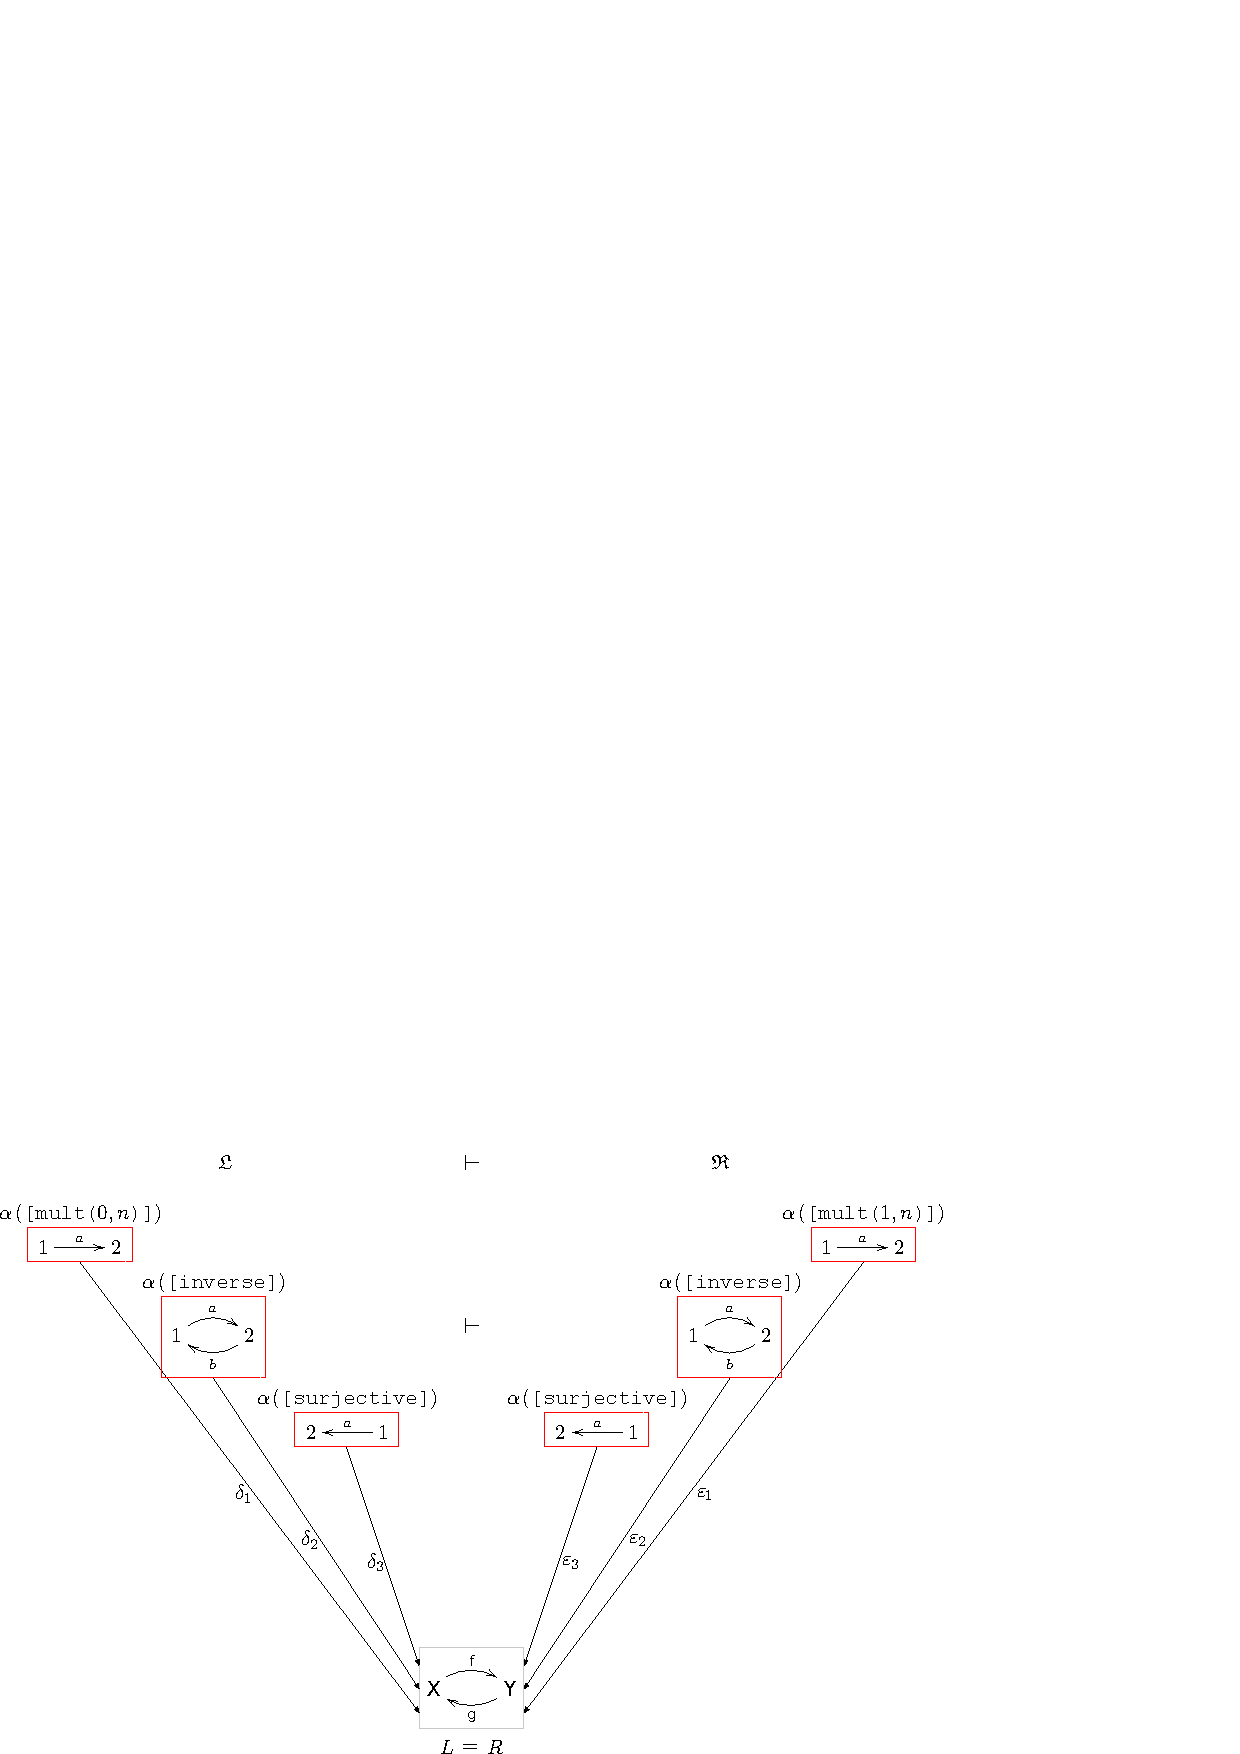
\includegraphics[width=\textwidth]{ex_spec_entailment}
  \end{center}
\end{frame}

\begin{frame}{Normalisation, custom conflict detection and resolution}
  \begin{center}
    \includegraphics<1>[scale=0.5]{ex_project_vc_custom_normalisation_md_md2_md3_2}
    \includegraphics<2>[scale=0.5]{ex_project_vc_custom_normalisation_md_md2_md3_3}
  \end{center}
\end{frame}

\begin{frame}{Complete synchronisation}
  \begin{center}
    \resizebox{\textwidth}{!}{
      $\xymatrix{
        & \spec{{UC}}[B] \ar@{_{(}->}[dl]_-{uinc_{\spec{U}[B]}} \ar[dr]^-{uinj_{\spec{V}[B]}} & & \spec{C}[B,H] \ar@{^{(}->}[drr]^-{inc_{\spec{V}[H]}} \ar[dl]_-{inj_{\spec{V}[B]}} & & & \spec{C}[H,H+1] \ar[dl]_-{inj_{\spec{V}[H]}}^-(0.4){}="r1" \ar@{^{(}->}[dr]^-{inc_{\spec{V}[H+1]}}_-(0.6){}="r2" \\
        \spec{U}[B] \ar@{_{(}->}[rd]_-{uinc_{\spec{{UD}}}} & \ar@{}[d]|-(0.2){P.O.} & \spec{V}[B] \ar[dl]^-{uinj_{\spec{{UD}}}} \ar[dr]_-{inj_{\spec{D}}} \ar@{}[dd]|-(0.6){P.O.} & \ldots \ar@{}[d]|-(0.2){P.O.} & & \spec{V}[H] \ar@{^{(}->}[lld]^-{inc_{\spec{D}}} & & \spec{V}[H+1] \\
        & \spec{{UD}} \ar[dr]_-{uinj_{\spec{{MD}}}} & & \spec{D} \ar[dl]^-{inj_{\spec{{MD}}}} & & & \spec{{UC}}[H] \ar[ul]_-(0.6){uinj_{\spec{V}[H]}}="l1" \ar@{^{(}->}[dr]^-(0.4){inc_{\spec{U}[H]}}="l2" \ar@{.>}[uu] \ar@{.>} "l1";"r1" \ar@{.>} "l2";"r2" \\
        & & \spec{{MD}} \ar[r]_-{se} & \spec{{MD'}} \ar@{^{(}->}[r]_-{cd} & \spec{{MD''}} \ar[r]_-{cr} & \spec{{MD'''}} & & \spec{U}[H] \ar[ll]^-{inj_{\spec{{MD'''}}}} \ar@{.>}[uu]
      }$
    }
  \end{center}
\end{frame}

\begin{frame}{Related work}
  Representation of differences
  \begin{itemize}
    \item {\textcolor{lily}{[\href{http://dx.doi.org/10.5381/jot.2007.6.9.a9}{Cicchetti et al., 2007}; \href{http://dx.doi.org/10.1007/978-3-540-69824-1\_9}{Rivera et al., 2008}]}} Difference metamodel
    \item {\textcolor{lily}{[\href{http://dx.doi.org/10.1145/940071.940102}{Ohst et al., 2003}]}} Annotations
    \item {\textcolor{lily}{[\href{http://dx.doi.org/10.1007/978-3-540-45221-8\_2}{Alanen et al., 2010}]}} Sequence of transformations
  \end{itemize}
\end{frame}

\begin{frame}{Related work}
  Model merging
  \begin{itemize}
    \item {\textcolor{lily}{[\href{http://dx.doi.org/10.1007/978-3-540-87875-9\_23}{Cicchetti et al., 2008}]}} Managing model conflicts in distributed development
    \item {\textcolor{lily}{[\href{http://dx.doi.org/10.1145/1826147.1826155}{Westfechtel, 2010}]}} A formal approach to three-way merging of EMF models
    \item {\textcolor{lily}{[\href{http://dx.doi.org/10.1007/978-3-642-15928-2\_12}{Taentzer et al., 2010}]}} Conflict detection for model versioning based on graph modifications
    \item {\textcolor{lily}{[\href{http://dx.doi.org/10.1007/978-3-642-13094-6\_28}{da Silva et al., 2010}]}} Towards automated inconsistency handling in design models
  \end{itemize}
\end{frame}

% \begin{frame}{Related work}
%   Heterogeneous synchronisation
%   \begin{itemize}
%     \item {\textcolor{lily}{[\href{http://dx.doi.org/10.1007/978-3-540-88643-3\_1}{Antkiewicz et al., 2008}]}} Design space of heterogeneous synchronization
%   \end{itemize}
%   Prototype tools
%   \begin{itemize}
%     \item {\textcolor{lily}{[\href{http://dx.doi.org/10.1057/palgrave.ejis.3000685}{DSMDiff}; \href{http://www.eclipse.org/emft/projects/compare/}{EMF Compare}]}} Differencing tools based on structural similarity
%     \item {\textcolor{lily}{[\href{http://www.modelversioning.org}{AMOR}]}} Centralised optimistic version control based on EMF
%   \end{itemize}
% \end{frame}



\section{Conclusion}

\begin{frame}{}
  \begin{center}
    \begin{Huge}
      \textbf{Conclusion}
    \end{Huge}
  \end{center}
\end{frame}

\begin{frame}{My contribution}
  Consolidation of DPF
  \begin{itemize}
    \item deleting transformation rules
    \item specification entailments
    \item prototype code generation
  \end{itemize}
\end{frame}

\begin{frame}{My contribution}
  Formal approach to model versioning
  \begin{itemize}
    \item complete work cycle
    \item calculation and representation of differences
    \item synchronisation
    \item constraint-awareness
  \end{itemize}
\end{frame}

\begin{frame}{My contribution}
  Formal approach to deep metamodelling
  \begin{itemize}
    \item semantics of double typing, linguistic extension and potency
    \item distinction of two semantics for potency
    \item flattening of deep characterisation of
  \end{itemize}
\end{frame}


\end{comment}


\begin{frame}{Thank you!}
  \vspace{5em}
  \begin{center}
    \begin{Huge}
      \textbf{Questions?\footnote{Courtesy to Alessandro Rossini for shareing introductory slides.}}
    \end{Huge}
  \end{center}
  \vspace{5em}
  %\begin{center}
  %  \href{http://dpf.hib.no}{dpf.hib.no}\\
  %  \href{http://www.alessandrorossini.org}{alessandrorossini.org}
  %\end{center}
\end{frame}

\end{document}
